%\documentclass[11pt]{article}
%\usepackage{graphicx}
%% This file is to hold any special settings for a particular CDR
% Things that are generic to CDRs in general go in cdr.cls.
% Probably no \usepackages should be here.

%\usepackage[pdftex,pdfpagelabels,bookmarks]{hyperref}



% This holds definitions of macros to enforce consistency in names.

% This file is the sole location for such definitions.  Check here to
% learn what there is and add new ones only here.  

% also see units.tex for units.

%%% Common terms

% Check here first, don't reinvent existing ones, add any novel ones.
% Use \xspace.

\def\expshort{LBN\xspace}
\def\explong{The Neutrino Experiment\xspace}

\def\anxlbnefd{Annex 4A: The LBNE Design for a Deep Underground Single-Phase Liquid Argon Time Projection Chamber\xspace}

% Things about oscillation
%
% example: \dm{12}
\newcommand{\dm}[1]{$\delta m^2_{#1}$\xspace}
% example \sinstt{12}
\newcommand{\sinstt}[1]{$\sin^22\theta_{#1}$\xspace}
% example \deltacp
\newcommand{\deltacp}{$\delta_{\rm CP}$\xspace}
% example \nuxtonux{\mu}{e}
\newcommand{\nuxtonux}[2]{$\nu_{#1} \to \nu_{#2}$\xspace}
\newcommand{\numutonumu}{\nuxtonux{\mu}{\mu}}
\newcommand{\numutonue}{\nuxtonux{\mu}{e}}
\newcommand{\numu}{$\nu_\mu$\xspace}
\newcommand{\nue}{$\nu_e$\xspace}
\newcommand{\anumu}{$\bar\nu_\mu$\xspace}
\newcommand{\anue}{$\bar\nu_e$\xspace}

% Names
\newcommand{\cherenkov}{Cherenkov\xspace}
\newcommand{\kamland}{KamLAND\xspace}
\newcommand{\kamiokande}{Kamiokande\xspace}
\newcommand{\superk}{Super--Kamiokande\xspace}
\newcommand{\miniboone}{MiniBooNE\xspace}
\newcommand{\minerva}{MINER$\nu$A\xspace}
\newcommand{\nova}{NO$\nu$A\xspace}
\newcommand{\SURF}{Sanford Underground Research Facility\xspace}


% This holds definitions of macros to enforce consistency in units.

% This file is the sole location for such definitions.  Check here to
% learn what there is and add new ones only here.  

% also see defs.tex for names.


% see
%  http://ctan.org/pkg/siunitx
%  http://mirrors.ctan.org/macros/latex/contrib/siunitx/siunitx.pdf

% Examples:
%  % angles
%  \ang{1.5} off-axis
%
%  % just a unit
%  \si{\kilo\tonne}
%
%  % with a value:
%  \SI{10}{\mega\electronvolt}

%  range of values:
% \SIrange{60}{120}{\GeV}

% some shorthand notation
\DeclareSIUnit \kton {\kilo\tonne}
\DeclareSIUnit \kt {\kilo\tonne}
\DeclareSIUnit \Mt {\mega\tonne}
\DeclareSIUnit \eV {\electronvolt}
\DeclareSIUnit \keV {\kilo\electronvolt}
\DeclareSIUnit \MeV {\mega\electronvolt}
\DeclareSIUnit \GeV {\giga\electronvolt}
\DeclareSIUnit \km {\kilo\meter}
\DeclareSIUnit \kW {\kilo\watt}
\DeclareSIUnit \MW {\mega\watt}
\DeclareSIUnit \MHz {\mega\hertz}
\DeclareSIUnit \mrad {\milli\radian}
\DeclareSIUnit \year {year}
\DeclareSIUnit \POT {POT}
\DeclareSIUnit \sig {$\sigma$}
\DeclareSIUnit\parsec{pc}
\DeclareSIUnit\lightyear{ly}
\DeclareSIUnit\foot{ft}
\DeclareSIUnit\ft{ft}
% for a bare kt-year
\def\ktyr{\si[inter-unit-product=\ensuremath{{}\cdot{}}]{\kt\year}\xspace}
\def\Mtyr{\si[inter-unit-product=\ensuremath{{}\cdot{}}]{\Mt\year}\xspace}
\def\msr{\si[inter-unit-product=\ensuremath{{}\cdot{}}]{\meter\steradian}\xspace}

\newcommand{\SIadj}[2]{\SI[number-unit-product = -]{#1}{#2}}
% Adjective form of some common units
% "the 10-kt detector"
\newcommand{\ktadj}[1]{\SIadj{#1}{\kt}}
% "the 1,300-km baseline"
\newcommand{\kmadj}[1]{\SIadj{#1}{\km}}
% "a 567-keV endpoint"
\newcommand{\keVadj}[1]{\SIadj{#1}{\keV}}
% "Typical 20-MeV event"
\newcommand{\MeVadj}[1]{\SIadj{#1}{\MeV}}
% "Typical 2-GeV event"
\newcommand{\GeVadj}[1]{\SIadj{#1}{\GeV}}
% "the 1.2-MW beam"
\newcommand{\MWadj}[1]{\SIadj{#1}{\MW}}
% "the 700-kW beam"
\newcommand{\kWadj}[1]{\SIadj{#1}{\kW}}
% "the 100-tonne beam"
\newcommand{\tonneadj}[1]{\SIadj{#1}{\tonne}}
% "the 4,850-foot depth beam"
\newcommand{\ftadj}[1]{\SIadj{#1}{\ft}}
%

% Mass exposure, people like to put dots between the units
% \newcommand{\ktyr}[1]{\SI[inter-unit-product=\ensuremath{{}\cdot{}}]{#1}{\kt\year}}
% must make usage of \ktyr above consistent with this one before turning on

% Beam x mass exposure, people like to put dots between the units
\newcommand{\ktmwyr}[1]{\SI[inter-unit-product=\ensuremath{{}\cdot{}}]{#1}{\kt\MW\year}}



% Set the major title, consistently across all volumes
\renewcommand\thevolumetitle{Conceptual Design Report \\ \explong}

% Do this here to make use of the experiment name and title macro
\hypersetup{
    pdftitle={\expshort CDR \thevolumesubtitle},
    pdfauthor={\expshort Collaboration},
    final=true,
    colorlinks=false,
    linktocpage=true,
    linkbordercolor=blue,
    citebordercolor=green,
    urlbordercolor=magenta,
    filecolor=black,
    pdfpagemode=UseOutlines,
    pdfborderstyle={/S/U},  
}




%\begin{document}
\chapter{Detector Development Program}
\label{ch:randd}

%\setlength{\parskip}{0.05in}

%%%%%%%%%%%%%%%%%%%%%%%%%%%%%%%%%%%%%%%%%%%%%%%%%%%%%%%%%%%%%%%%%%%
\section{Introduction}
This chapter describes the development program designed to ensure a successful and cost-effective construction and operation of the massive, dual-cryostat LArTPC detector for LBNE and to investigate possibilities for enhancing the performance of the detector. The feasibility of the LArTPC as a detector has been demonstrated most impressively by the ICARUS experiment. \fixme{add ref?}

It is understood that for successful operation an LArTPC has stringent requirements on
\begin{itemize}
 \item argon purity, which must be of order 200~ppt O$_2$ equivalent or better
 \item long-term reliability of components located within the liquid argon; in particular, the TPC and field cage must be robust against wire-breakage and must support a cool-down of over 200~K
 \item the front-end electronics, which must achieve a noise level ENC of $1000 e$ or better
\end{itemize}

The design of the LBNE LArTPC has evolved significantly from earlier concepts based on standard, above-ground, upright cylindrical LNG storage tanks which envisioned single TPC sense and high-voltage planes spanning the full width of the tank -- essentially a direct scaling of previous detectors. Problems with the actual construction of such massive planes and with the logistics of being able to construct the TPC only after the cryostat was complete are avoided in the present design. In this design,  TPC `panels'  are fully assembled and tested  --- including the electronics ---  independently of the cryostat construction. This modular approach is a key feature of the design. It has the benefit not only of improving the logistics of detector construction, but also the individual components can be of manageable size. It should also be noted that the cryostat itself is formed of modular panels designed for quick and convenient assembly.

This chapter does not provide a comprehensive overview of the liquid argon detector development
efforts worldwide; it discusses several that are closely related to the LBNE detector, including the Material
Test System, TPC design, the 35-t membrane cryostat prototype at Fermilab and its testing program, 
and the single-phase prototype detector proposed for construction at CERN.

%%%%%%%%%%%%%%%%%%%%%%%%%%%%%%%%%%%%%%%%%%%%%%%%%%%%%%%%%%%%%%%%%%%
% section on components of program removed per Jim Stewart

%%%%%%%%%%%%%%%%%%%%%%%%%%%%%%%%%%%%%%%%%%%%%%%%%%%%%%%%%%%%%%%%%%%
\section{Materials Test System}
\label{sec:mts}


An area for LAr detector development, shown in Figure~\ref{fig:PAB}, has been established in the Proton Assembly Building at Fermilab. The Materials Test System (MTS) has been developed to determine the effect on electron-drift lifetime of materials and components that are candidates for 
inclusion in LAr-FD. The system essentially consists 
of a source of clean argon ($<30$ ppt O$_{2}$ equivalent), a cryostat, a sample chamber that can be purged or evacuated,  a mechanism for transferring a sample from the sample chamber into the cryostat, a mechanism for setting the sample height in the cryostat so that it can be placed either in the liquid or in the gas ullage above the liquid, a temperature probe to measure the temperature of the sample, and an electron-lifetime monitor. The system is fully automated and the lifetime data are stored in a single database along with the state of the cryogenic system. 

\begin{cdrfigure}[Liquid argon area at the Proton Assembly Building at Fermilab]{PAB}{Liquid argon area at the Proton Assembly Building at Fermilab}
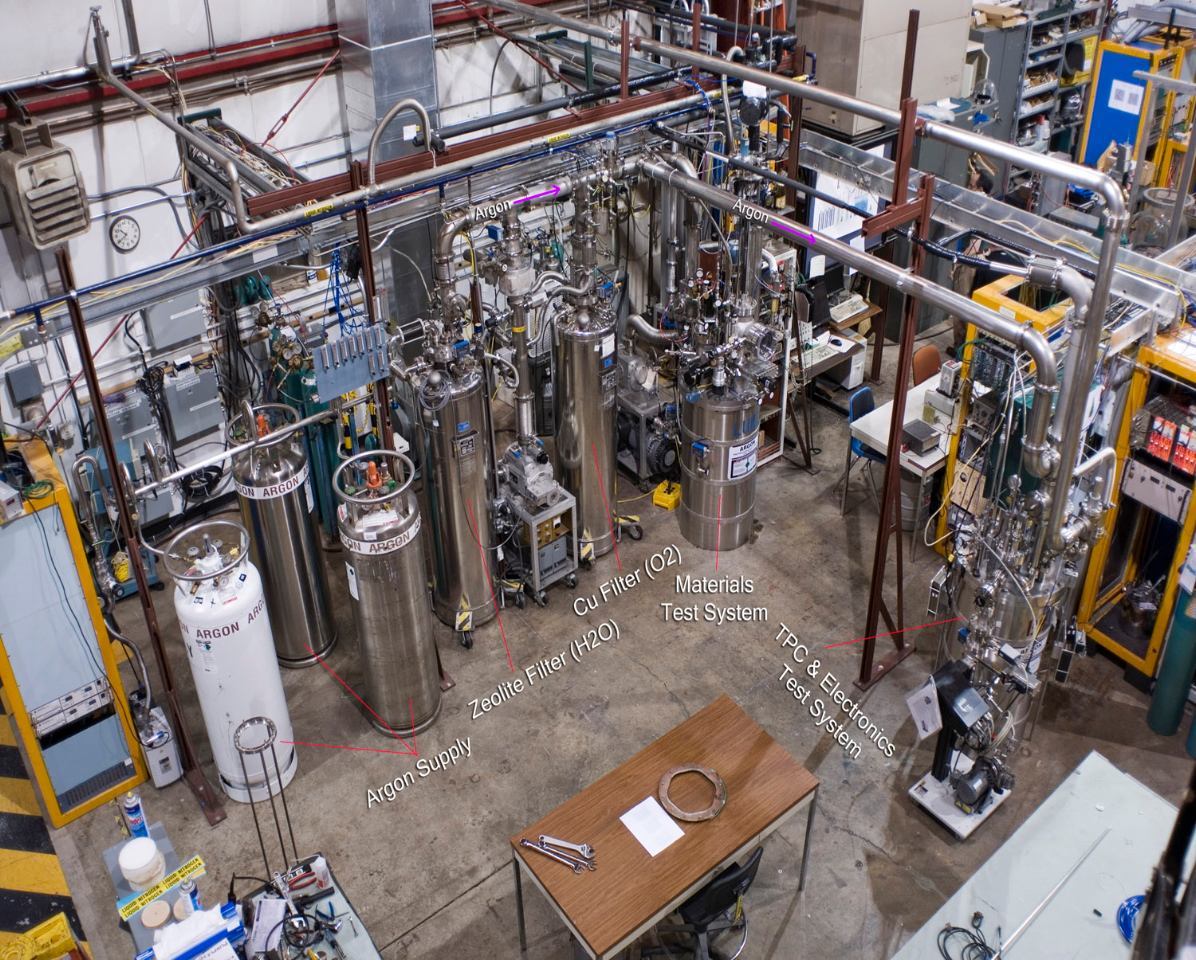
\includegraphics[width=0.8\textwidth]{LAratPAB.pdf}
\end{cdrfigure}

A noteworthy feature is the novel bubble-pump filter inside the cryostat. In case of argon contamination, this can filter the cryostat volume in a few hours, allowing continuation of studies 
 without having to refill. A schematic of the MTS is shown in Figure~\ref{fig:MTS_Schem}.

\begin{cdrfigure}[Schematic of the Materials Test System (MTS) cryostat at Fermilab]{MTS_Schem}{Schematic of the Materials Test System (MTS) cryostat at Fermilab}
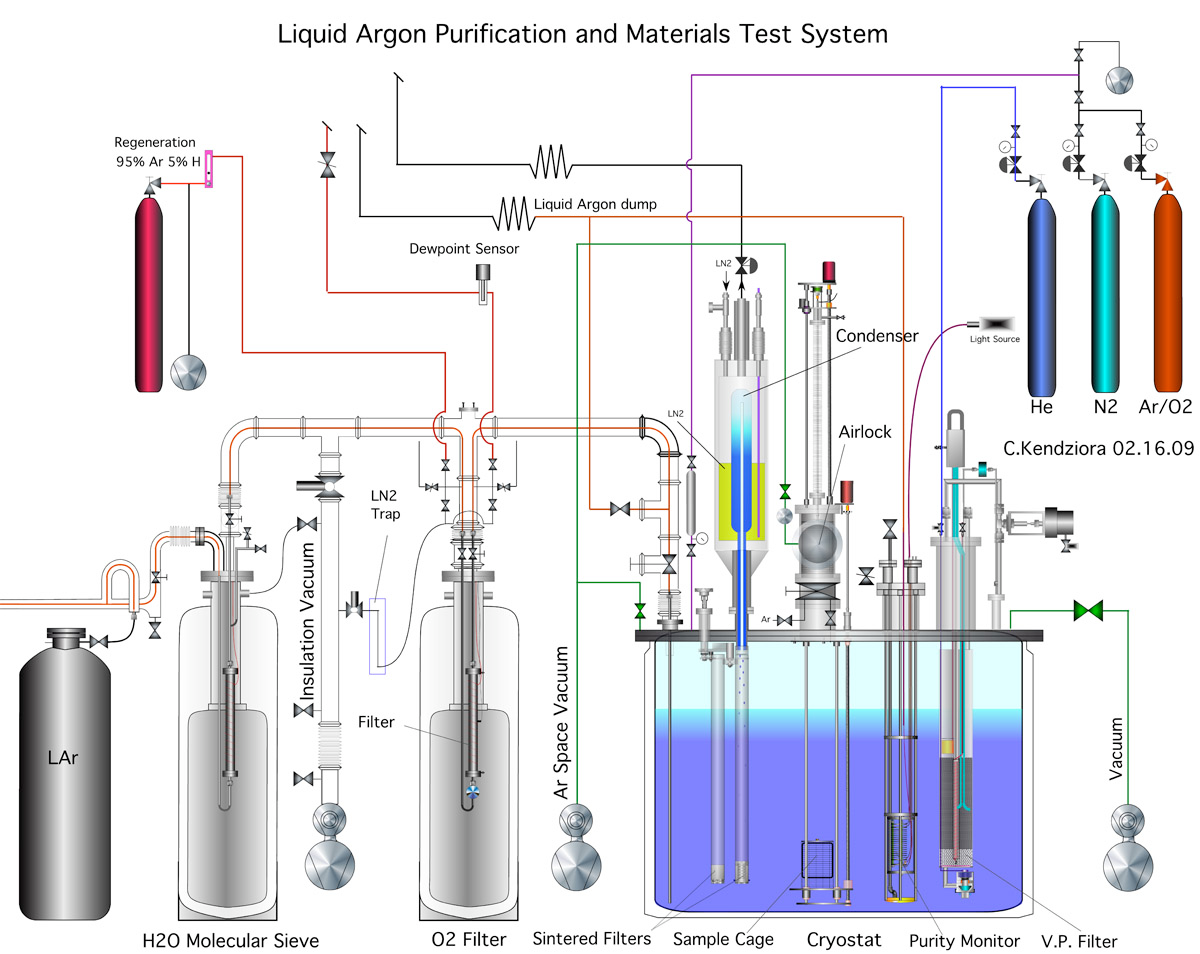
\includegraphics[width=0.9\textwidth]{MTS_Full_Schematic.pdf}
\end{cdrfigure}

The major conclusions of the studies are summarized here. No material has been found that affects the electron-drift lifetime when the material is immersed in liquid argon -- this includes, for example, the common G-10 substitute, FR-4. On the other hand, materials in the ullage can contaminate the liquid; this contamination is dominated by the water outgassed by the materials and as a result is strongly temperature-dependent. Any convection currents that transport water-laden argon into the LAr and any cold surfaces on which water-laden argon can condense will fall into the LAr and reduce the electron lifetime. Conversely,  a steady flow of gaseous argon of a few ft/hr away from the LAr prevents any material in the gas volume from contaminating the LAr. 

These results are taken into account in the design of both MicroBooNE and LAr-FD. For LBNE they have been cast as detector requirements. The MTS will continue to be used by MicroBooNE and LBNE to test detector materials such as cables that will reside in the ullage.


%%%%%%%%%%%%%%%%%%%%%%%%%%%%%%%%%%%%%%%%%%%%%%%%%%%%%%%%%%%%%%%%%%%
\section{TPC Design}

A string of recent events in several liquid argon setups, such as Long Bo, DarkSide50, ArgonTube and MicroBooNE, in which the sustainable high voltage (HV) was much lower  than designed voltages,  prompted a reevaluation of the breakdown strength of liquid argon, especially at ``detector grade'' purity. Recent studies \cite{bib:HV_in_LAr_1}\cite{bib:HV_in_LAr_2} have revealed that the HV-breakdown strength depends on factors such as electrode feature size, distance, stress area/volume, and LAr purity. Although no conclusive threshold was found, the results indicate that the safe operating field in LAr is well under 100~kV/cm. 
 
With the uncertainty in the liquid argon HV dielectric strength, attention will be focused on the HV-related aspects of the TPC design involving the CPAs and field cage modules.  An R\&D document has been compiled for the far detector~\cite{fd_rndplan_10006} that contains a section on the proposed R\&D topics and activities to reduce the HV-related risks. Apart from the HV feedthrough, which will be designed and tested above the operating voltages, there is a plan to improve the designs of the CPAs and field cage modules.
 
The current TPC design directly interconnects all CPAs on a cathode plane. Two of the outer cathode planes face the grounded cryostat walls. The stored energy between one of the outer cathode planes and the cryostat wall, with the full bias voltage applied, is more than 150 joules\cite{ve-fd_025_8920}. This amount of energy, if released suddenly in an event of a high voltage discharge, is sufficient to raise the temperature of a cube of stainless steel with 2-mm sides by 4000$^\circ$K, resulting in a leak in the membrane cryostat. Moreover, a sudden collapse of the cathode voltage will also inject very large current pulses into the front-end ASICs connected to the first induction plane wires, causing damage to the electronics.
 
To minimize these risks, the logical steps are:
\begin{itemize}
\item minimize the stored energy when possible by swapping the locations of the APA and CPA planes such that no CPAs are against the cryostat wall.
\item slow the voltage collapse in a discharge by constructing the cathode planes out of highly resistive material to form a long RC time constant for discharge
\begin{itemize}
\item study the electrical behavior of CPAs constructed from highly resistive material
\item identify and test a resistive coating that is robust at cryogenic temperature and able to maintain good adhesion to the cathode structure
\item design the new CPAs with all resistive elements
\end{itemize}
\end{itemize}
 
Techniques for applying a highly resistive coating over the current 35t-style printed circuit board-based panels on the field cage are being developed in order to remove field concentration around the conductor edges.
%On the field cage, we are developing the techniques to apply a highly resistive coating over the current 35t-style printed circuit board-based panels to remove field concentration around the conductor edges. 
In parallel, a fall back solution for reducing the field using roll-formed electrodes with a much larger edge radius is being developed.
 
For the APAs, a simple and effective method to contain a broken outer layer wire must be developed; such a wire must be prevented from drifting far into the drift volume and making contact with the field cage.
 

%%%%%%%%%%%%%%%%%%%%%%%%%%%%%%%%%%%%%%%%%%%%%%%%%%%%%%%%%%%%%%%%%%%
\section{35-ton Prototype: Phase 1}
\label{35tonprototype}

When first conceived, the 35t prototype cyrostat was constructed to demonstrate that a non-evacuable membrane cryostat can satisfy the less-than-200-parts-per-trillion (ppt) requirement on oxygen contamination of the liquid argon in the detector and maintain that level stably.
%
It was intended to prototype a wide variety of issues that construction and 
operation of the far detector would need to address, including procurement of 
materials and services, safety and the processes involved with ensuring the 
cryostat can maintain high-purity liquid argon. 
%
Later it was decided to extend its scope, and to install and operate a small-scale LArTPC and photon detector in the cryostat; this phase will focus on the performance of active detector elements placed directly in the volume of liquid argon.

The membrane cryostat demonstration, completed in 2014, is referred to as ``Phase 1'' and the operation of the TPC is called ``Phase 2.''
Phase 2 is currently under construction and it is planned to take data in summer 2015.

\fixme{Needed a bit more introduction before going into the details; I added info above. Please check.}


\subsection{Phase 1 Construction}
\label{sec:rnd:35t1:construction}

The construction of the 35t cryostat addressed a number of issues.
First were project-related issues, such as gaining detailed construction experience, 
developing the procurement and contracting model, and incorporating the design and approval mechanism 
in the Fermilab ES\&H manual, which was necessary because membrane cryostats are designed in accordance
with European and Japanese standards.
Secondly, it addressed technical issues such as %demonstrating 
high-purity operation in this type of 
cryostat and the suitability of the planned LAr-FD construction techniques and materials.

The LBNE project contracted with the Japanese company IHI to build the 35t cryostat at Fermilab.  
It was built in Fermilab's PC-4 facility where the Liquid Argon Purity Demonstrator (LAPD)
\cite{bib:lapdP07005}
is also located, which
allowed for re-use of a large portion of the cryogenic-process equipment installed for LAPD.
The proximity and size (30 tons) of LAPD also offers the possibility using LAPD as 
a partial storage vessel for LAr if the 35t ever needs to be emptied. 
The 35t employs a submersible %LAr 
pump to pump the LAr from the cryostat to the filters. Two pumps were installed for redundancy, but 
only one is used at a time.
Figure~\ref{fig:35cryo} shows the layout of the 35t prototype at 
Fermilab's PC-4 facility. 
Figure~\ref{fig:35cutaway} shows a cutaway view of the cryostat and a photograph of the interior
of the completed cryostat. 

\begin{cdrfigure}[35t prototype at Fermilab's PC-4 facility, layout]{35cryo}{Layout of 35t prototype at Fermilab's PC-4 facility. }
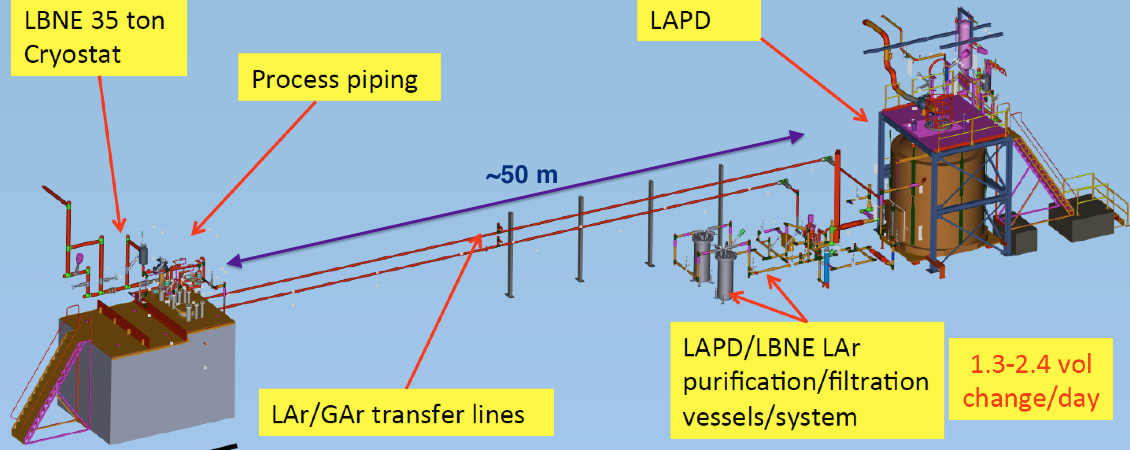
\includegraphics[width=0.9\textwidth]{35TLayout}
\end{cdrfigure}

\begin{cdrfigure}[35t Cutaway view]{35cutaway}{(left) Cutaway view of the 35t cyrostat; (right) Interior
photograph of the completed cryostat.}
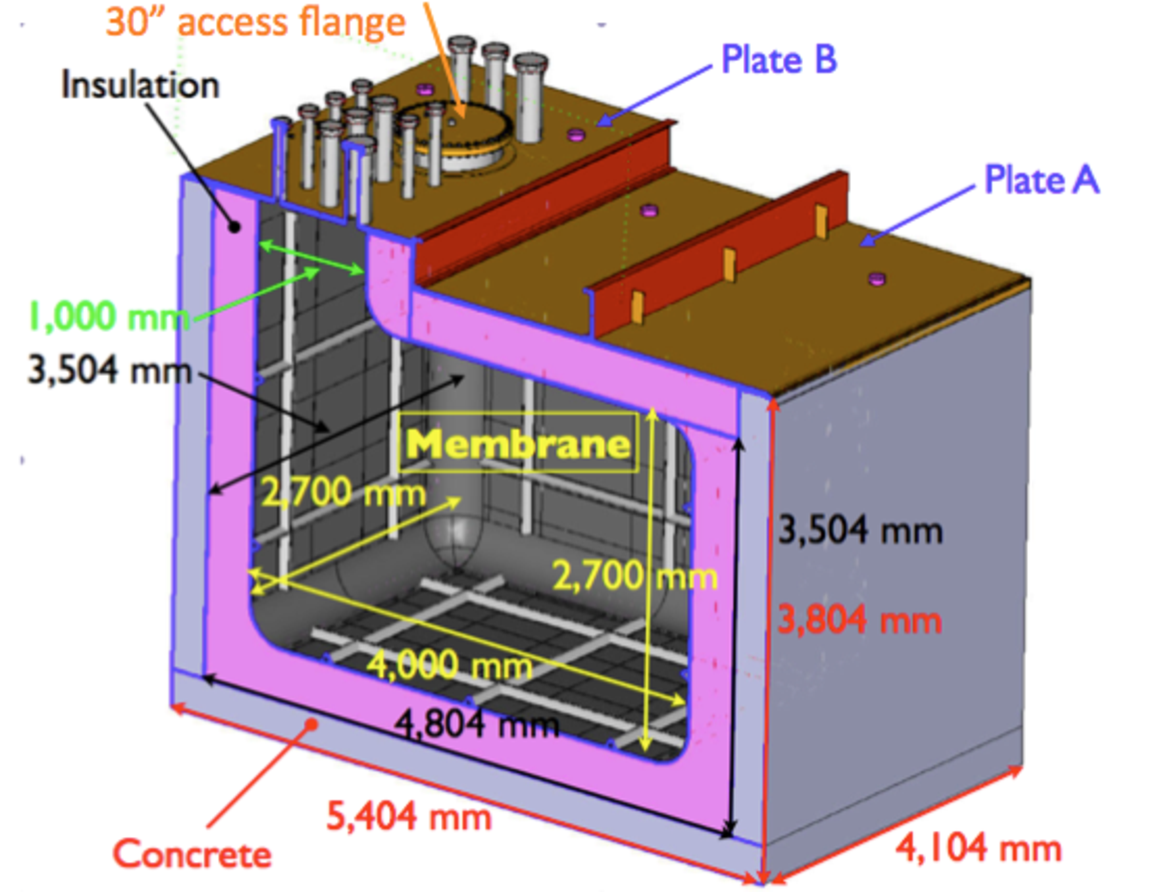
\includegraphics[width=0.60\textwidth]{35TCutaway}
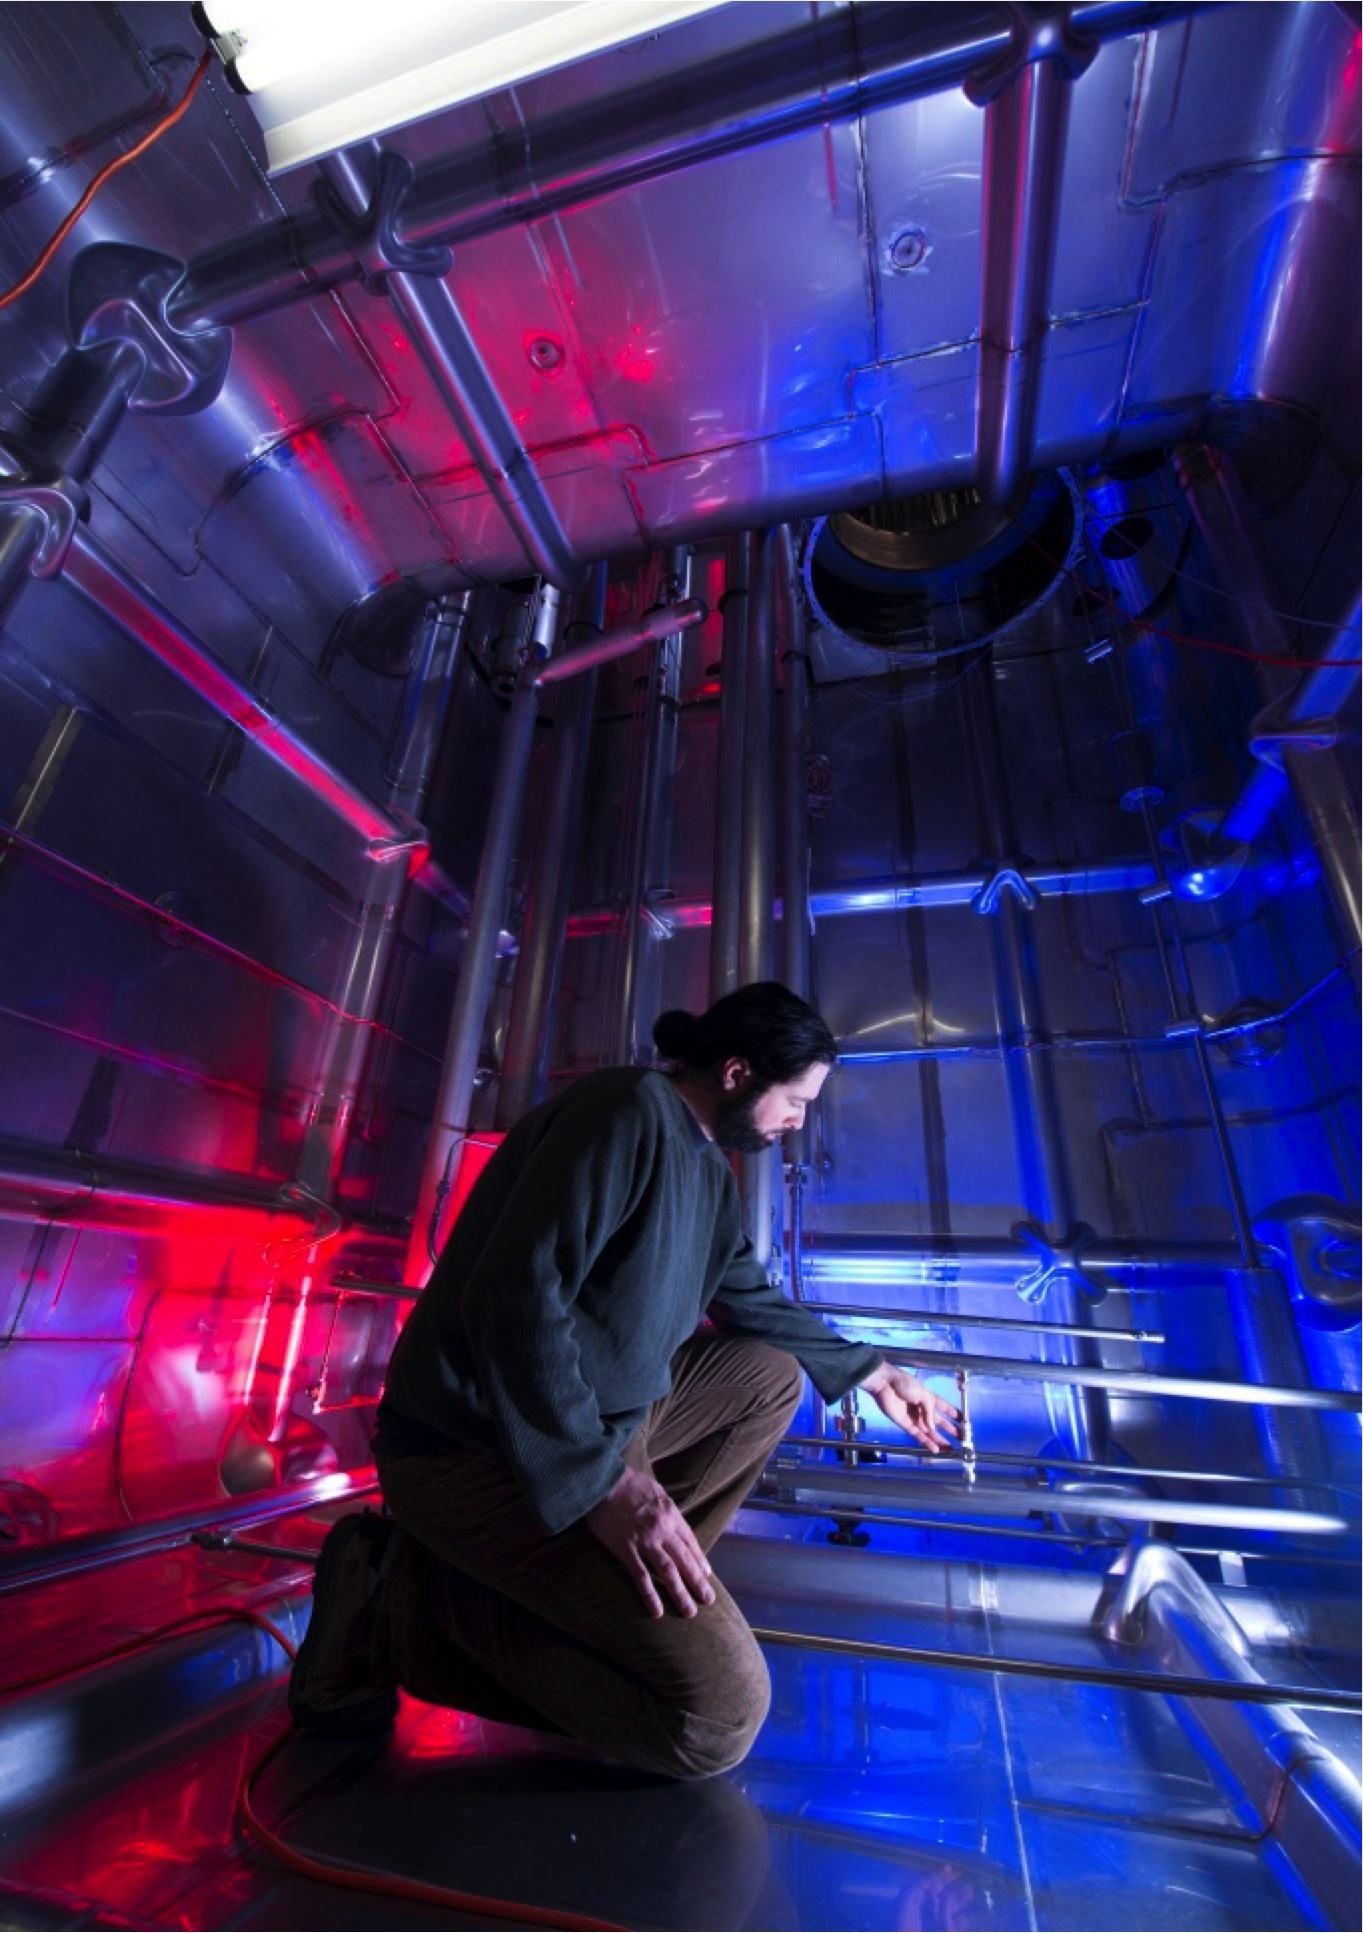
\includegraphics[width=0.35\textwidth]{35TCryo}
\end{cdrfigure}

Table~\ref{tab:35Tdimensions} gives the details of the construction materials and the
dimensions for the 35t.
More information can be found in
\cite{bib:membcryo1573}.
The insulation thickness is 0.4~m rather than the 1.0~m chosen for the reference design.  
The techniques of membrane-cryostat construction were demonstrated to be a fit 
for high-purity TPC service.
Welding of corrugated panels, removal of leak-checking dye penetrant or ammonia-activated
leak-detecting paints, and post-construction-cleaning methods were tested for suitability of service.  

\begin{cdrtable}[35t Details and Dimensions]{ll}{35Tdimensions}
{35t Details and Dimensions}
Parameter & Value \\ \toprowrule
Cryostat Volume	&      29.16 m3\\ \colhline
Liquid Argon total mass	 &     38.6 metric tons\\ \colhline
Inner dimensions	&      4.0 m (L) x 2.7 m (W) x 2.7 m (H)\\ \colhline
Outer dimensions        &      5.4 m (L) x 4.1 m (W) x 4.1 m (H)\\ \colhline
Membrane		&      2.0 mm thick corrugated 304 SS\\ \colhline
Insulation		&      0.4 m polyurethane foam\\ \colhline
Secondary barrier system	   &   0.1 mm thick fiberglass\\ \colhline
Vapor barrier	Normal	  &    1.2 mm thick carbon steel\\ \colhline
Steel reinforced concrete	    &  0.3 m thick layer\\ 
\end{cdrtable}

%Residual contamination measurements at different elevations during the initial GAr purge process 
%will be compared to computational predictions and will validate the purge-process modeling of a
%large rectangular vessel. 
%The prototype membrane cryostat will be filled with LAr.  
%Purity levels of the liquid with time and electron-drift times will be measured using purity 
%monitors installed in the liquid bath.  Heat-load measurements will be made and compared to 
%calculations. 
%Eventually, connectors and feedthroughs, ports and other features that are planned for the 
%reference design will be incorporated into the prototype.  
%Materials and cold-electronics testing can be done along with electron-drift-time measurements.

In principle, a thin-walled membrane cryostat is as suitable as a thick-walled cryostat
for use with high-purity LAr. 
Both are constructed with 304 stainless steel with a polished surface finish.
Both use passive insulation. 
The total length of interior welds required for construction would be similar in both cases.
The leak-checking procedure would be the same in both cases.

The significant difference between membrane cryostats and thick-walled cryostats is
the depth of the welds used to construct the vessel.  
The majority of membrane-cryostat welds are completed in one or two passes with 
automatic welding machines. 
A second difference, and a major advantage, is that the membrane cryostat is a standard
industrial design that has been in use for over 40 years. 
A thick-walled cryostat vessel would be custom designed and would require significant 
engineering and testing. 
A third difference, and another major advantage, is the ability to purge the membrane 
cryostat insulation space with argon gas so that a leak cannot affect the purity if 
it escapes detection and repair. 

%A 3-m $\times$ 3-m wall panel shown in Figure~\ref{fig:3panel} was constructed at Fermilab
%using materials and technical guidance from GTT. 
%The labor hours used in construction are consistent with the vendor estimates. The wall panel was leak tested (none we%re found) and vacuum tests were performed on the insulation system. We found that the insulation system is designed to% allow vacuum pumping of the main cryostat volume to a hard vacuum. This result demonstrates that vacuum pumping of a %membrane cryostat is feasible, if it is found to be required. No modifications to the vendor-supplied components are r%equired to accomplish this.


%\begin{cdrfigure}[Membrane panel assembly and components]{3panel}{Membrane panel assembly and components}
%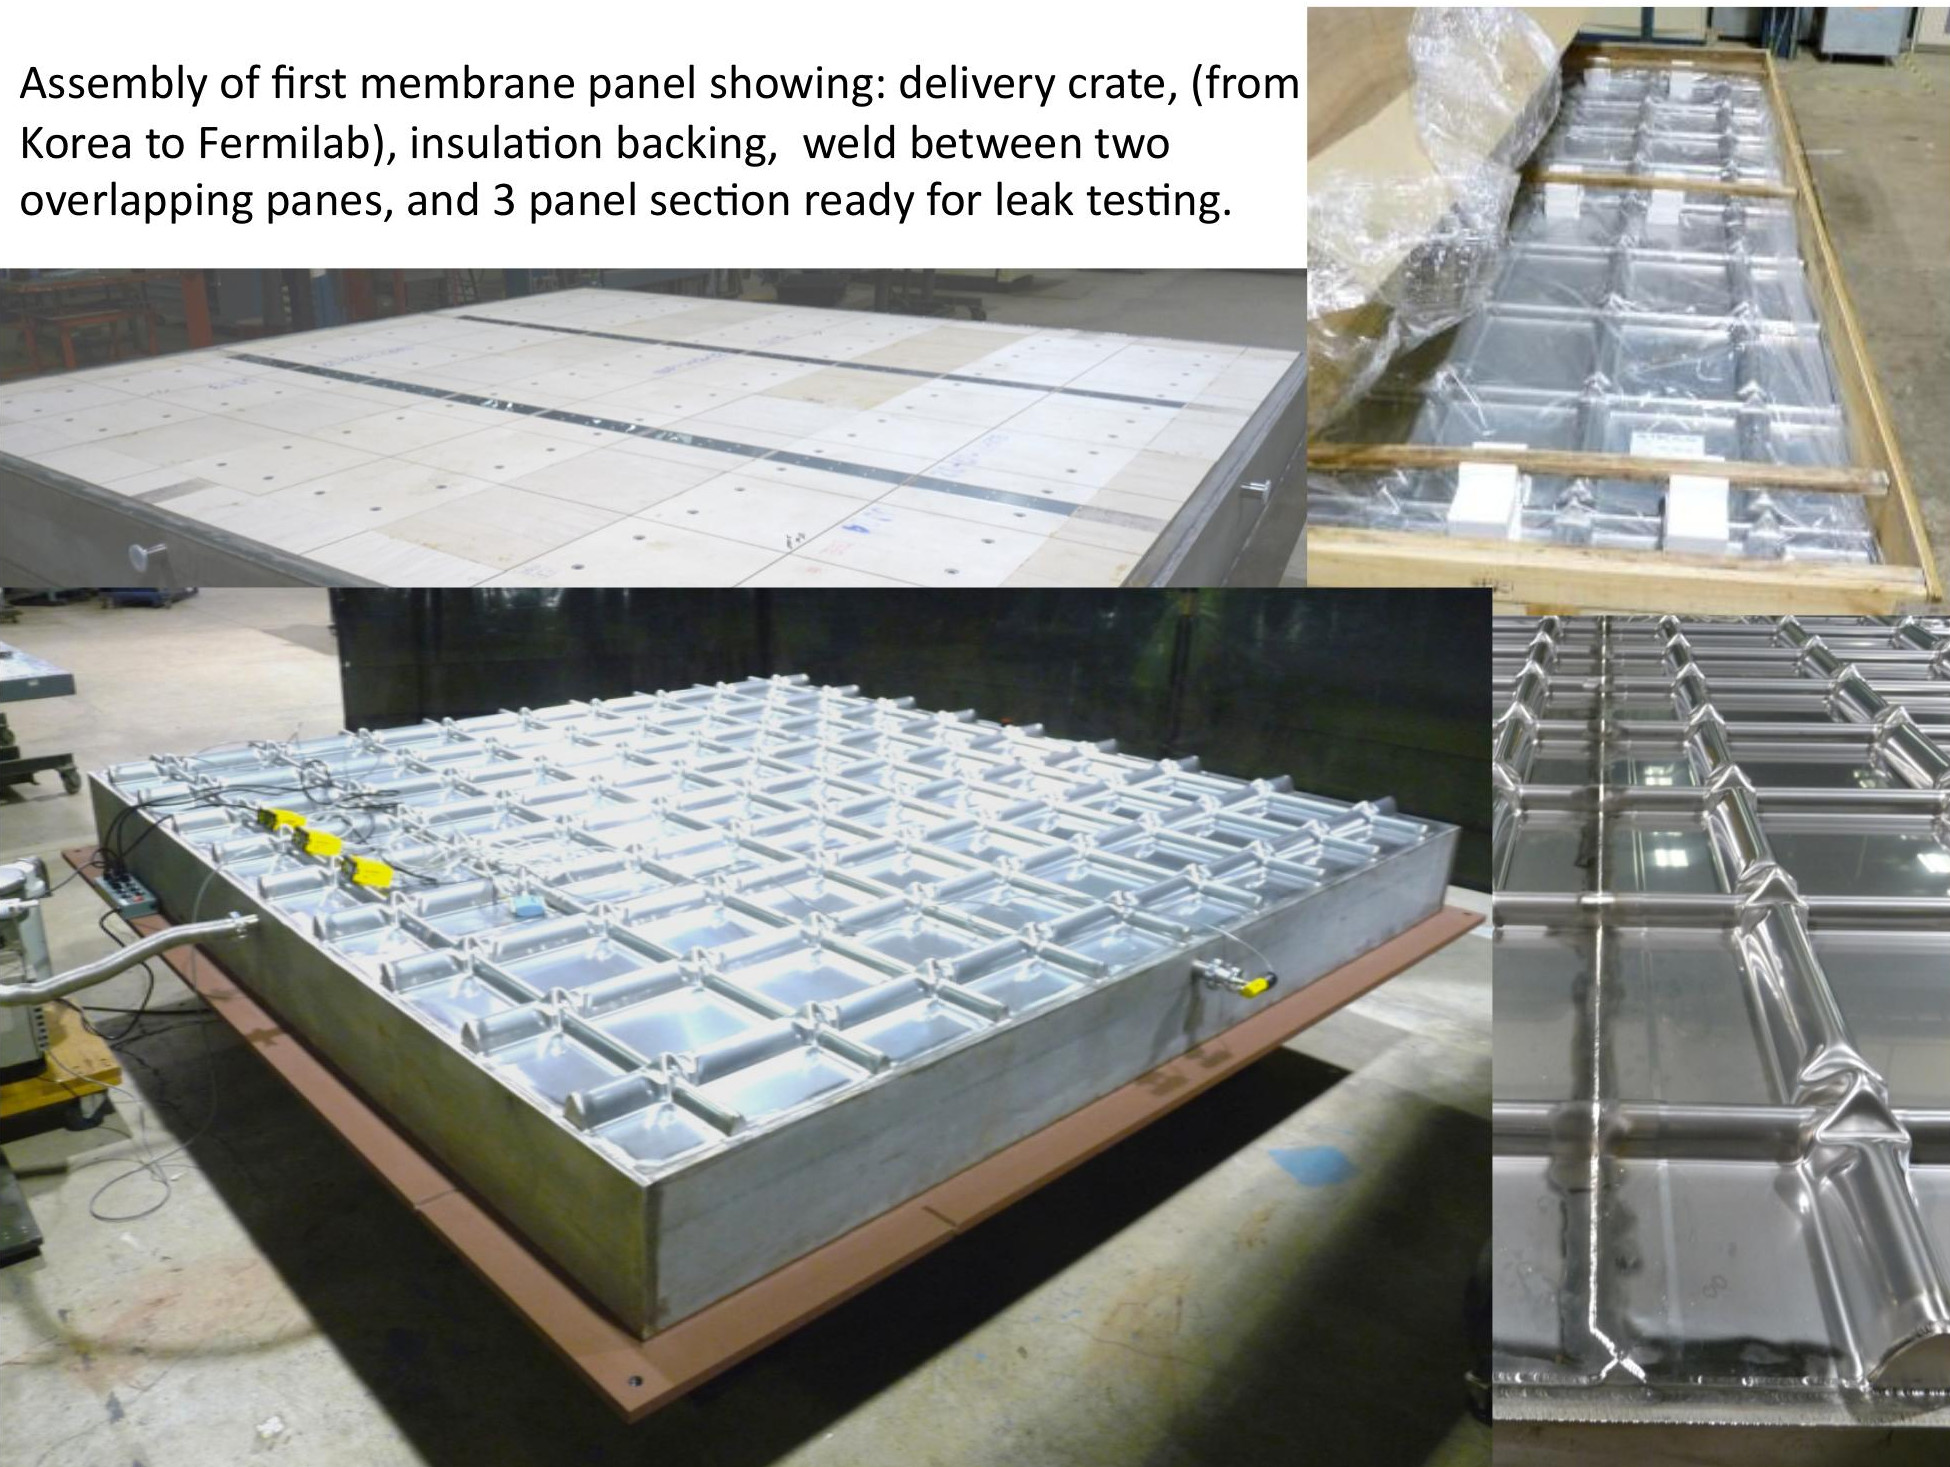
\includegraphics[width=0.7\textwidth]{Membranepastichepage}
%\end{cdrfigure}

%\begin{cdrfigure}[35T Cryostat]{35Cryo}{Interior view of the completed 35T cryostat.}
%\includegraphics[width=0.7\textwidth]{35cryo.png}
%\end{cdrfigure}

\subsection {Phase 1 Cryogenics Instrumentation}

The 35t includes a full complement of standard commercial transducers and sensors that are used to 
monitor and control the cryogenic environment. They include temperature sensors, pressure transducers 
(absolute and gauge), flow meters, and level sensors. These devices are typically read out directly into the 
Control System and data-logged. 

A number of commercial gas analyzers measure trace impurity levels (O$_2$, H$_2$O, and 
N$_2$) in the argon. Some have sensitivities at the 100 ppt level. A gas distribution switchyard feeding the 
gas analyzers allows the sampling points in the 35t to be reconfigured.

There were also two purpose-built pieces of instrumentation for the monitoring of the high-purity 
LAr environment,   % needed for a LAr detector. They are 
the purity monitors (PrMs) and the RTD Spooler. The 
PrMs are used to measure electron lifetimes in the LAr, and the RTD Spooler is used to make precision 
measurements of the temperature profile of the cryostat as a function of depth.  These instruments were 
originally constructed for the LAPD run and are fully described %in depth 
in \cite{bib:lapdP07005}.

%%%%%%%%%%%%%%%%%%%%%%%%%%%%
\subsection {Phase 1 Operations}

\fixme{This needs an initial sentence stating what the operations are, e.g., air purge, cooldown/fill, LAr purification. I added the following, please check}

The operational portion of Phase 1 involved three main steps: 

\begin{enumerate}
\item{removal of the air from the cryostat, leaving only Ar gas (the Piston Purge)}
\item cooldown and fill of the cryostat with high-purity LAr
\item maintenance of the high purity level of the LAr
\end{enumerate}

The first two steps above are part of the purification process, which also involves 
%In order to purify LAr, it is necessary to do three things:  
\begin{enumerate}
\item{cleaning the liquid Ar as it comes from the supplier}
\item{removal of any impurities that are generated by materials outgassing within the cryostat.}
\end{enumerate}
  
LAPD, referred to in Section~\ref{sec:rnd:35t1:construction},
 had already demonstrated that it is not necessary to evacuate a cryostat in order achieve 
LAr purity levels sufficient for LBNE. \fixme{something about `but it didn't demonstrate
it for the type of cryostat planned for use in the far detector ...' In other words, why did we still need the 35t for phase 1?}
This is of paramount importance since the costs of multi-kiloton cryostats that 
could withstand evacuation is prohibitive. 
The 35t followed the procedure LAPD~\cite{bib:lapdP07005}
established to obtain and maintain pure LAr. 

%%%%%%%%%%%%%%
\subsubsection {Gas Phase}

%The initial state of the 35t was that 
When the phase 1 test began, ``dry'' air had been purging the cryostat for approximately three weeks. 

The first step of the ``gas phase'' portion of the process, the Piston Purge, removes the air in the cryostat; during this step argon gas is flooded into the bottom of the cryostat. Since argon is heavier than air, the argon layer rises, analogous to a mechanical piston, pushing the air up and out of the cryostat. This gas \fixme{initially 100\% air?} is vented to the outside atmosphere. The venting stage continues for 32 hours, approximately the equivalent of 12 volume changes. 
%
Figure~\ref{fig:35TPurge} graphically shows step 1 of the purification process, removal of the ambient air. The initial state, $t=0$, reflects the initial values for oxygen, water and nitrogen in the ``dry air'' state. This is followed by the Piston Purge.
These measurements are made by a variety of %gas 
monitors that sample the gas in the cryostat. 

\begin{cdrfigure}[35t Gas Ar Purge and Recirculation]{35TPurge}{Gas phase of removing impurities in the 35t. These quantities are being measured by various gas analyzers. The first stage of the purification is a process called the ``Piston Purge''.  The second stage is ``Recirculation with Filtering''. The gap between the two steps was due to troubleshooting a leak.}
  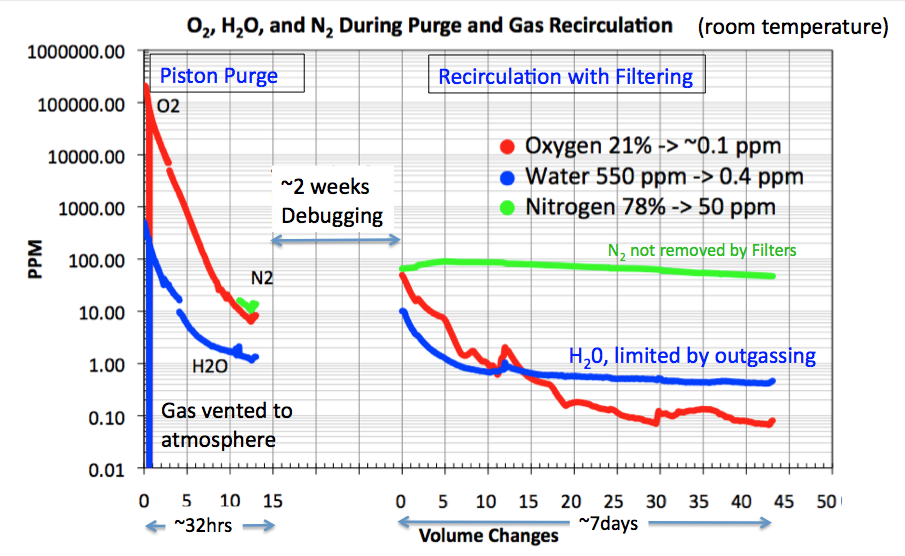
\includegraphics[width=\textwidth]{35TPurgeAndRecirc}
\end{cdrfigure}


%At this point 
After the purge, the exiting gas \fixme{which is mostly/all argon?} is re-routed to circulate through the filtration system that removes O$_2$ and H$_2$O. (N$_2$ is not materially removed by the filters.) Any leaks to the outside atmosphere can be detected during this step. As shown in ``Debugging'' gap in Figure~\ref{fig:35TPurge}, a leak was found and mitigated. Once leaks have been eliminated the recirculation continues until the O$_2$ level drops to the sub-ppm level. As can be seen in the plot, the H$_2$O level plateaus at a much higher level than O$_2$. This is due to the outgassing of materials inside the 35t, including the cryostat walls, which are \fixme{remain?} at room temperature during \fixme{throughout?} the recirculation step. 

%%%%%%%%%%%%%%
\subsubsection {Cooldown and LAr Fill}

\begin{cdrfigure}[35t Cooldown and Fill]{35TCooldown}{Cooldown and filling the 35t. The 
measurements (red trace) are made from RTDs afixed to the cryostat walls. The black dashed curve is the 
manufacturer's maximum allowed cooldown rate. The filling (blue trace) was from the transfer of LAr 
from LAPD, This quantity of LAr is less than the capacity of the 35t. The RTD traces drop to the LAr 
temperature when the level of the LAr covers reaches their mounting height.}
  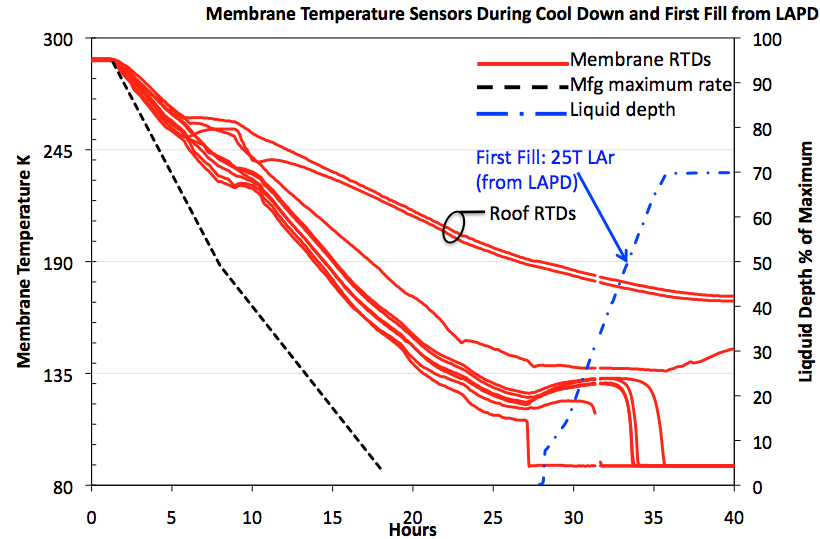
\includegraphics[width=\textwidth]{35TCoolDown.png}
\end{cdrfigure}

A gas/liquid spray method is used to cool down the cryostat. This generates a turbulent mixing 
of cold gas in the cryostat and cools the entire surface. The cooldown rate was %limited to be less than 
maintained lower (slower) than
the maximum rate specified by the membrane cryostat manufacturer. The cooldown, as well as the initial 
fill, is shown in Figure~\ref{fig:35TCooldown}. The temperature measurements (red traces) in this plot 
were made by RTDs that are glued to the membrane walls of the cryostat. The black dashed trace is the 
manufacturer specification for the cooldown rate.

Once the cooldown was complete, the LAr transfer into the cryostat began. % In the case of the 35t phase 1 run, 
In this case the LAr came from LAPD, where it had been used by that system in its own recently completed 
second run\cite{bib:lapdP07005}. 

LAPD contained about 30 tons of LAr, of which only 25 tons could be transferred to the 35t providing a$\sim$70\% fill. It was decided to begin the initial commissioning of the 
Phase 1 run at this point since several components of the 35t could be commissioned at this fill level. After running with the partial fill for approximately eighteen days, additional LAr was 
added to bring the capacity to 100\%, the full 35 tons.

%%%%%%%%%%%%%%
\subsubsection{LAr Purification}

The Fermilab Material Test System (MTS)\cite{bib:Voiron9940,bib:mtslapd308} (see Section~\ref{sec:mts}) has shown that contaminants released inside LAr-filled cryostats come from materials outgassing in the warm ullage regions above the LAr surface. Typical detector materials submersed in LAr have negligible impact of LAr purity levels. \fixme{only because the materials have to be tested for this, right?}

Figure~\ref{fig:35TVaporFlow} depicts how impurities generated by outgassing materials in the 
relatively warm ullage under Plate B are swept up by the normal Ar boil-off in the 35t. This impure vapor 
is condensed in the LN$_2$-cooled LAr condensor. The impure condensate is returned to the 35t just inside 
the intake manifold of the interior submersible LAr pump. From there it is pumped to the filtration 
system where the impurities are removed.

%Of interest, 
It is worth noting that the electron lifetime of \fixme{`in'?} the LAr exiting the filters, as measured by the inline PrM was always  
> 30 ms (corresponding to a purity $\sim$10 ppt O$_2$ equivalent). This indicates that the filters are very efficient at removing all 
trace amounts of O$_2$ and H$_2$O. This was true for the entire 35t phase 1 run, including the filling periods.

\begin{cdrfigure}[35t Vapor Flow]{35TVaporFlow}{Drawing of Boiloff/Outgassing Vapor Flow (white 
arrows) from the 35t cryostat, with condensate return (violet arrows) from the condensor into the Pump 
Intake Manifold. LAr flow into the pump, and return from the Purification filters are shown by blue 
arrows. Also shown is the location of the Stainless Steel Radiation baffles beneath Plate B. This location 
just beneath Plate B is the warmest location and presumably the principal source of outgassing within the 
cryostat.}
  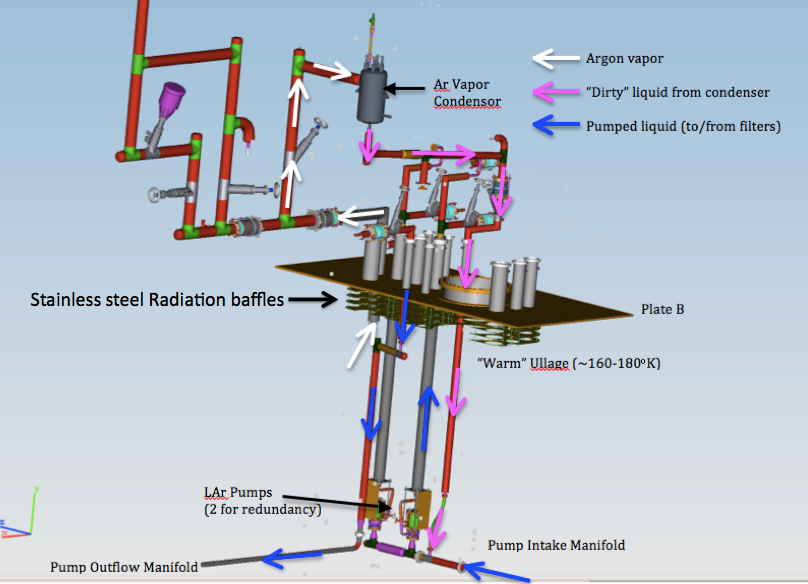
\includegraphics[width=\textwidth]{35TVaporFlow.png}
\end{cdrfigure}

Figure~\ref{fig:35TElectronLifetime} plots the electron lifetime from the start of the LAr Pump operation until the end of the Phase 1 run. In general, the electron lifetime improved as a function of pump 
``on-time,'' but %there were several 
a few incidents, shown on the plot, %that spoiled 
impacted the lifetime. These will be discussed in the next section.

%%%%%%%%%%%%%%%%%%%%%%%%%%%%
\subsection {Phase 1 Stability of Operation}

The goals of the 35t Phase 1 run included not only achieving the required purity/lifetime levels, but to 
also hold those levels and provide \fixme{demonstrate?} a stable operation of the cryostat. The 35t Phase 1 LAr run lasted a relatively 
short $\sim$2 months.% of LAr running. 
Electron lifetimes in the 2-3 ms range were achieved, as can be seen in 
Figure~\ref{fig:35TElectronLifetime}.

The electron lifetimes were severely impacted, however, whenever one LAr pump would switch to 
another. The drops in purity coincided with the turn on of the previously-inactive pump (see annotations 
in Figure~\ref{fig:35TElectronLifetime}). The issue is believed to lie with the procedure used to start the 
pumps; it will be modified for future operations in the 35t Phase 2 run.

A second stability question is keeping the temperature stable in the cryostat. Currently the 35t controls 
system regulates the gauge pressure of the cryostat, keeping the internal pressure to 6.69(02) kPa above 
ambient atmospheric pressure. However this leaves the thermodynamics of the LAr sensitive to normal 
atmospheric pressure changes.

\begin{cdrfigure}[35t Electron Lifetime]{35TElectronLifetime}{LAr electron lifetmes as measured by 
Cryostat Purity Monitors. Significant events are annotated on the plot. Major divisions on horizontal axis 
are one week periods. Equivalent purity levels are shown as dashed horizontal lines.}
  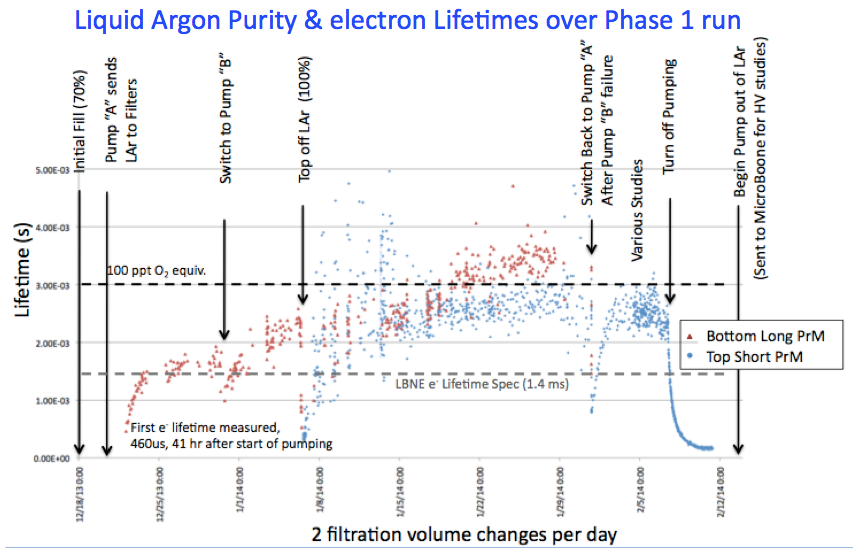
\includegraphics[width=\textwidth]{35TElectronLifetime.png}
\end{cdrfigure}

Figure~\ref{fig:35TTempStability} shows a plot over a nine-day period of the cryostat absolute pressure (blue 
trace), bulk LAr temperature (white dashed trace) and the normalized drift time of three PrMs, one short 
and long inside the cryostat, and the long inline PrM exterior to the cryostat. The temperature is taken 
from the RTD Spooler measurements by requiring that the RTDs be at least 15 cm below the LAr surface. \fixme{prev sentence doesn't make sense to me. You take a temperature by
requiring some condition to be in place?}
The temperature curve lags the pressure changes ($\Delta P \sim~3.5$~kPa over this period) due to the thermal 
inertia of the LAr. However \fixme{is `however' right? what's the contrast?} the normalized drift time (= drift time/(average drift time for this period) is 
directly correlated to the LAr temperature. The LAr temperature excursion range was $\Delta T \sim~0.3$~K. 
Fitting the normalized drift velocity (inverse of normalized drift time) gives the result 

% won't compile $\Delta_{\fract{driftspeed}{\overline{driftspeed}}} = -\fract{0.022}{001}~K$\\

 $\Delta_{driftspeed/\overline{driftspeed}} = -0.022/001~K$\\
 
The electron drift velocities for these three PrMs varied from (0.3 to 0.4) mm/$\mu$s depending on the individual PrM's drift field. 

\begin{cdrfigure}[35t Temperature Stability]{35TTempStability}{Interior Cryostat Absolute Pressure 
(blue trace), bulk LAr temperature (white dashed trace), and PrM drift times (dots) over a nine-day period. 
Major divisions on horizontal axis are one day intervals. The PrM drift times are from three PrMs, two in 
the cryostat, and the third from the inline PrM. The lag between the temperature and pressure is due to 
the thermal inertia of the LAr.}
  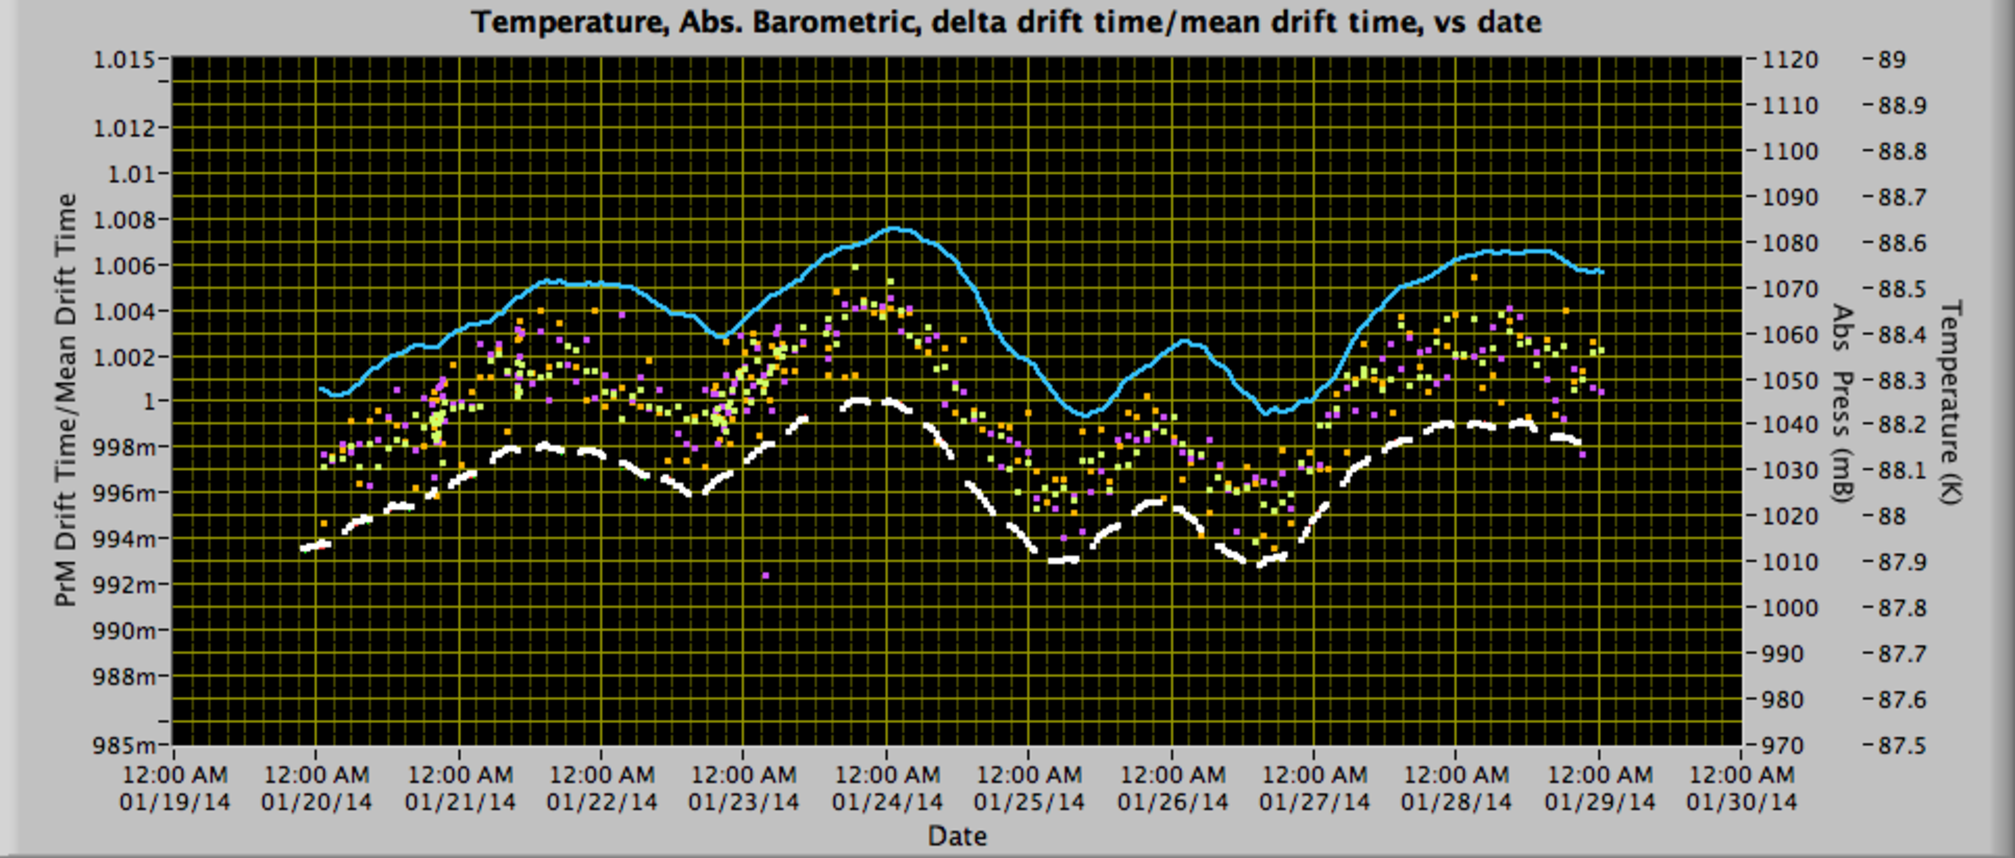
\includegraphics[width=\textwidth]{35TTempStability}
\end{cdrfigure}

The RTD Spooler was intended to provide a precision measurement of the vertical temperature profile. 
This measurement is a means of testing the Computational Fluid Dynamics Simulations [5]\fixme{what is actual reference?} that 
are being made on the fluid motion in the cryostat. Experimentally measuring the actual motion does not 
appear to be feasible at this time. The CFD calculations are being used to understand whether there 
might be dead areas in the cryostat where impurities might collect. Figure~\ref{fig:SpoolerScan} shows the result of one RTD 
scan. This scan was taken from a period where the barometric pressure was relatively constant so that 
the temperature would remain constant during the scan. Since a scan takes up to 6 hours in one direction 
(up or down) and as can be seen in Figure~\ref{fig:35TTempStability}, pressure changes can impact the 
bulk temperature of the LAr. These profiles seen in Figure~\ref{fig:SpoolerScan} are in nominal 
agreement with the current CFD calculations [5]\fixme{add real reference, same as the one above?}.


\begin{cdrfigure}[35t Vertical Temperature Profile]{SpoolerScan}{(top) RTD Spooler Vertical Temperature scan of the 35t Cryostat under Plate B showing both the liquid and vapor temperature.  (bottom) Expanded horizontal axis around 88.12~K. Note that the horizontal divisions on the lower plot are 50~mK. }
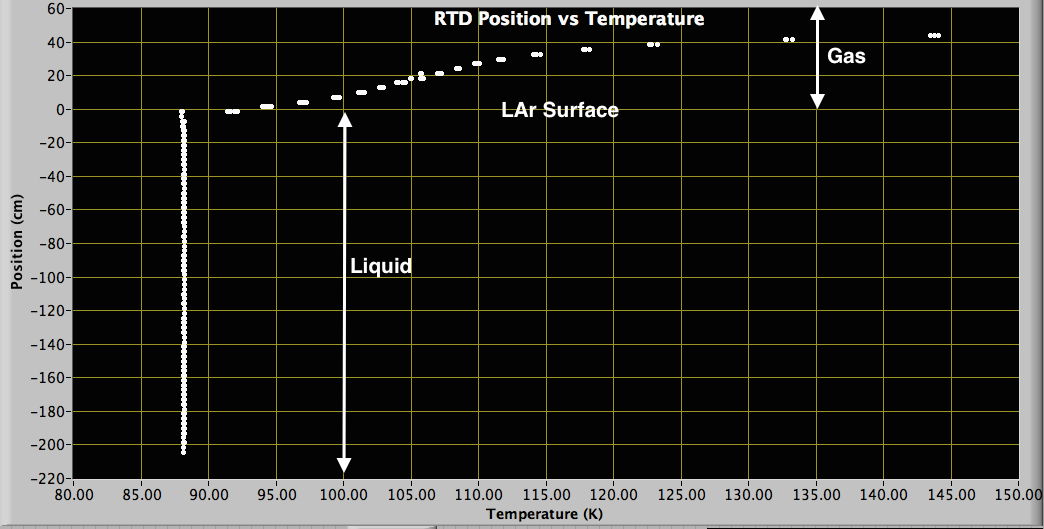
\includegraphics[width=\textwidth]{SpoolerScanFull.png}
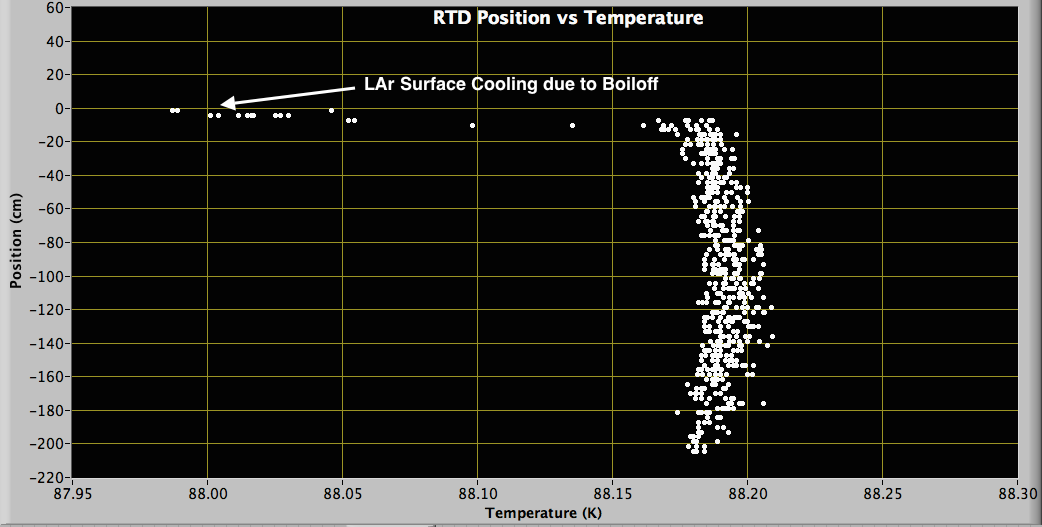
\includegraphics[width=\textwidth]{SpoolerScanExpand.png}  
\end{cdrfigure}

\subsection{Phase 1 Conclusions}

The 35t Phase 1 run has shown that the membrane cryostat technology has no innate difficulties with 
achieving the stated goals of the LBNE Conceptual Design Far Detector. Some of the 35t issues (e.g., loss 
of purity when pumps are switched) are most likely unique to the 35t. It also seems likely that in a future 
design, the pumps will be externally located, to avoid coupling acoustical vibrations into the Far Detector 
cryostat and to facilitate maintenance and repair.

%%%%%%%%%%%%%%%%%%%%%%%%%%%%%%%%%%%%%%%%%%%%%%%%%%%%%%%%%%%%%%%%%%%
\section{35t Prototype Phase 2}

Phase 2 of the the 35t prototype involves installing a fully operational TPC and photon detector into 
the previously built cryostat.
The prototype will be filled with liquid argon and operated for a several-month-long cosmic ray run. 
External plastic scintillator paddles placed around the cryostat will be used to produce
trigger signals as well as rough position measurements of the incoming cosmic rays.
Installation of the TPC into the cryostat is expected in April 2015 and 
commissioning is expected to begin in June 2015.
%Figure~\ref{fig:tpc-35ton-trial} shows the trial assembly of the TPC outside of the cryostat. 
Figure~\ref{fig:35TTPC} shows a model of the TPC inside the cryostat and a trial assembly of
the TPC done outside of the cyrostat. 

\subsection{35t Phase 2 TPC Design}

\begin{cdrfigure}[35t with TPC]{35TTPC}{(left) 35t Cryostat with TPC and photon detectors installed. 
Note separate drift regions on ``near'' and ``far'' sides.
The near side drift length is close to what is proposed for the far detector. The far
side has a shorter drift length due to lack of space.
(right) A trial assembly of the TPC.
}
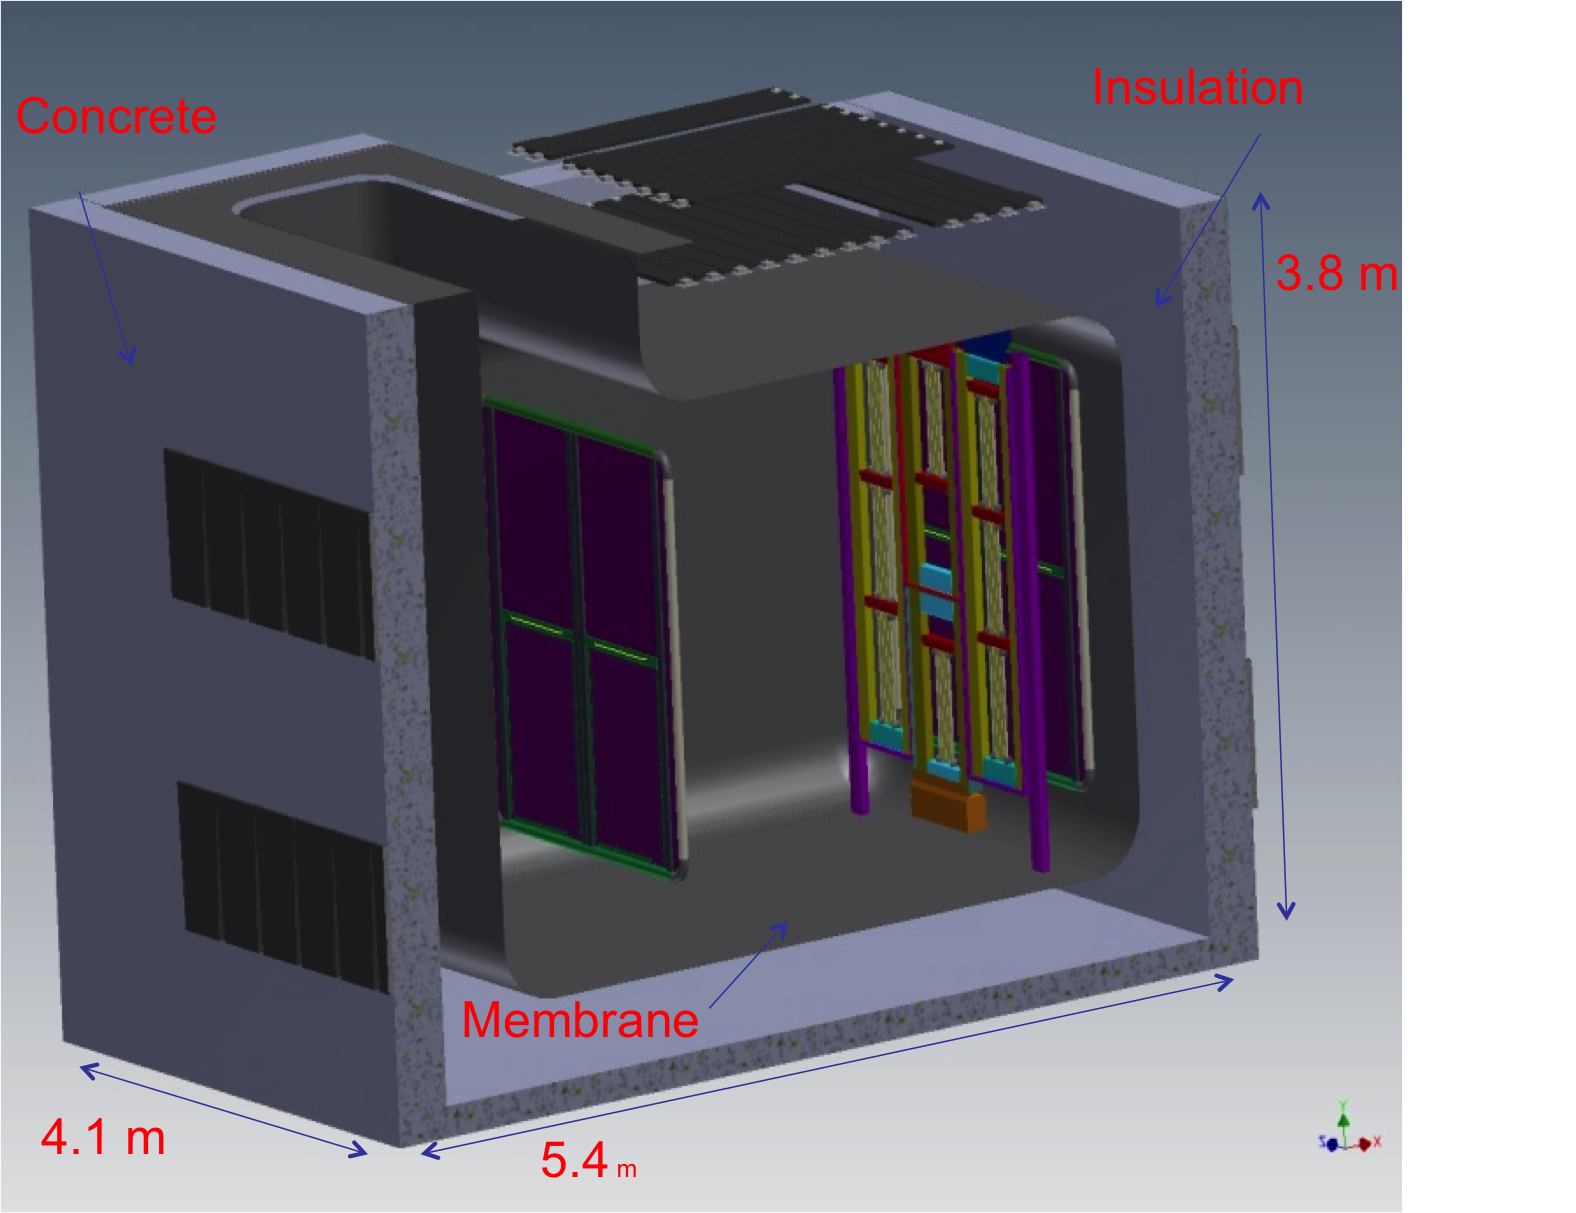
\includegraphics[width=0.55\textwidth]{35TTPC}  
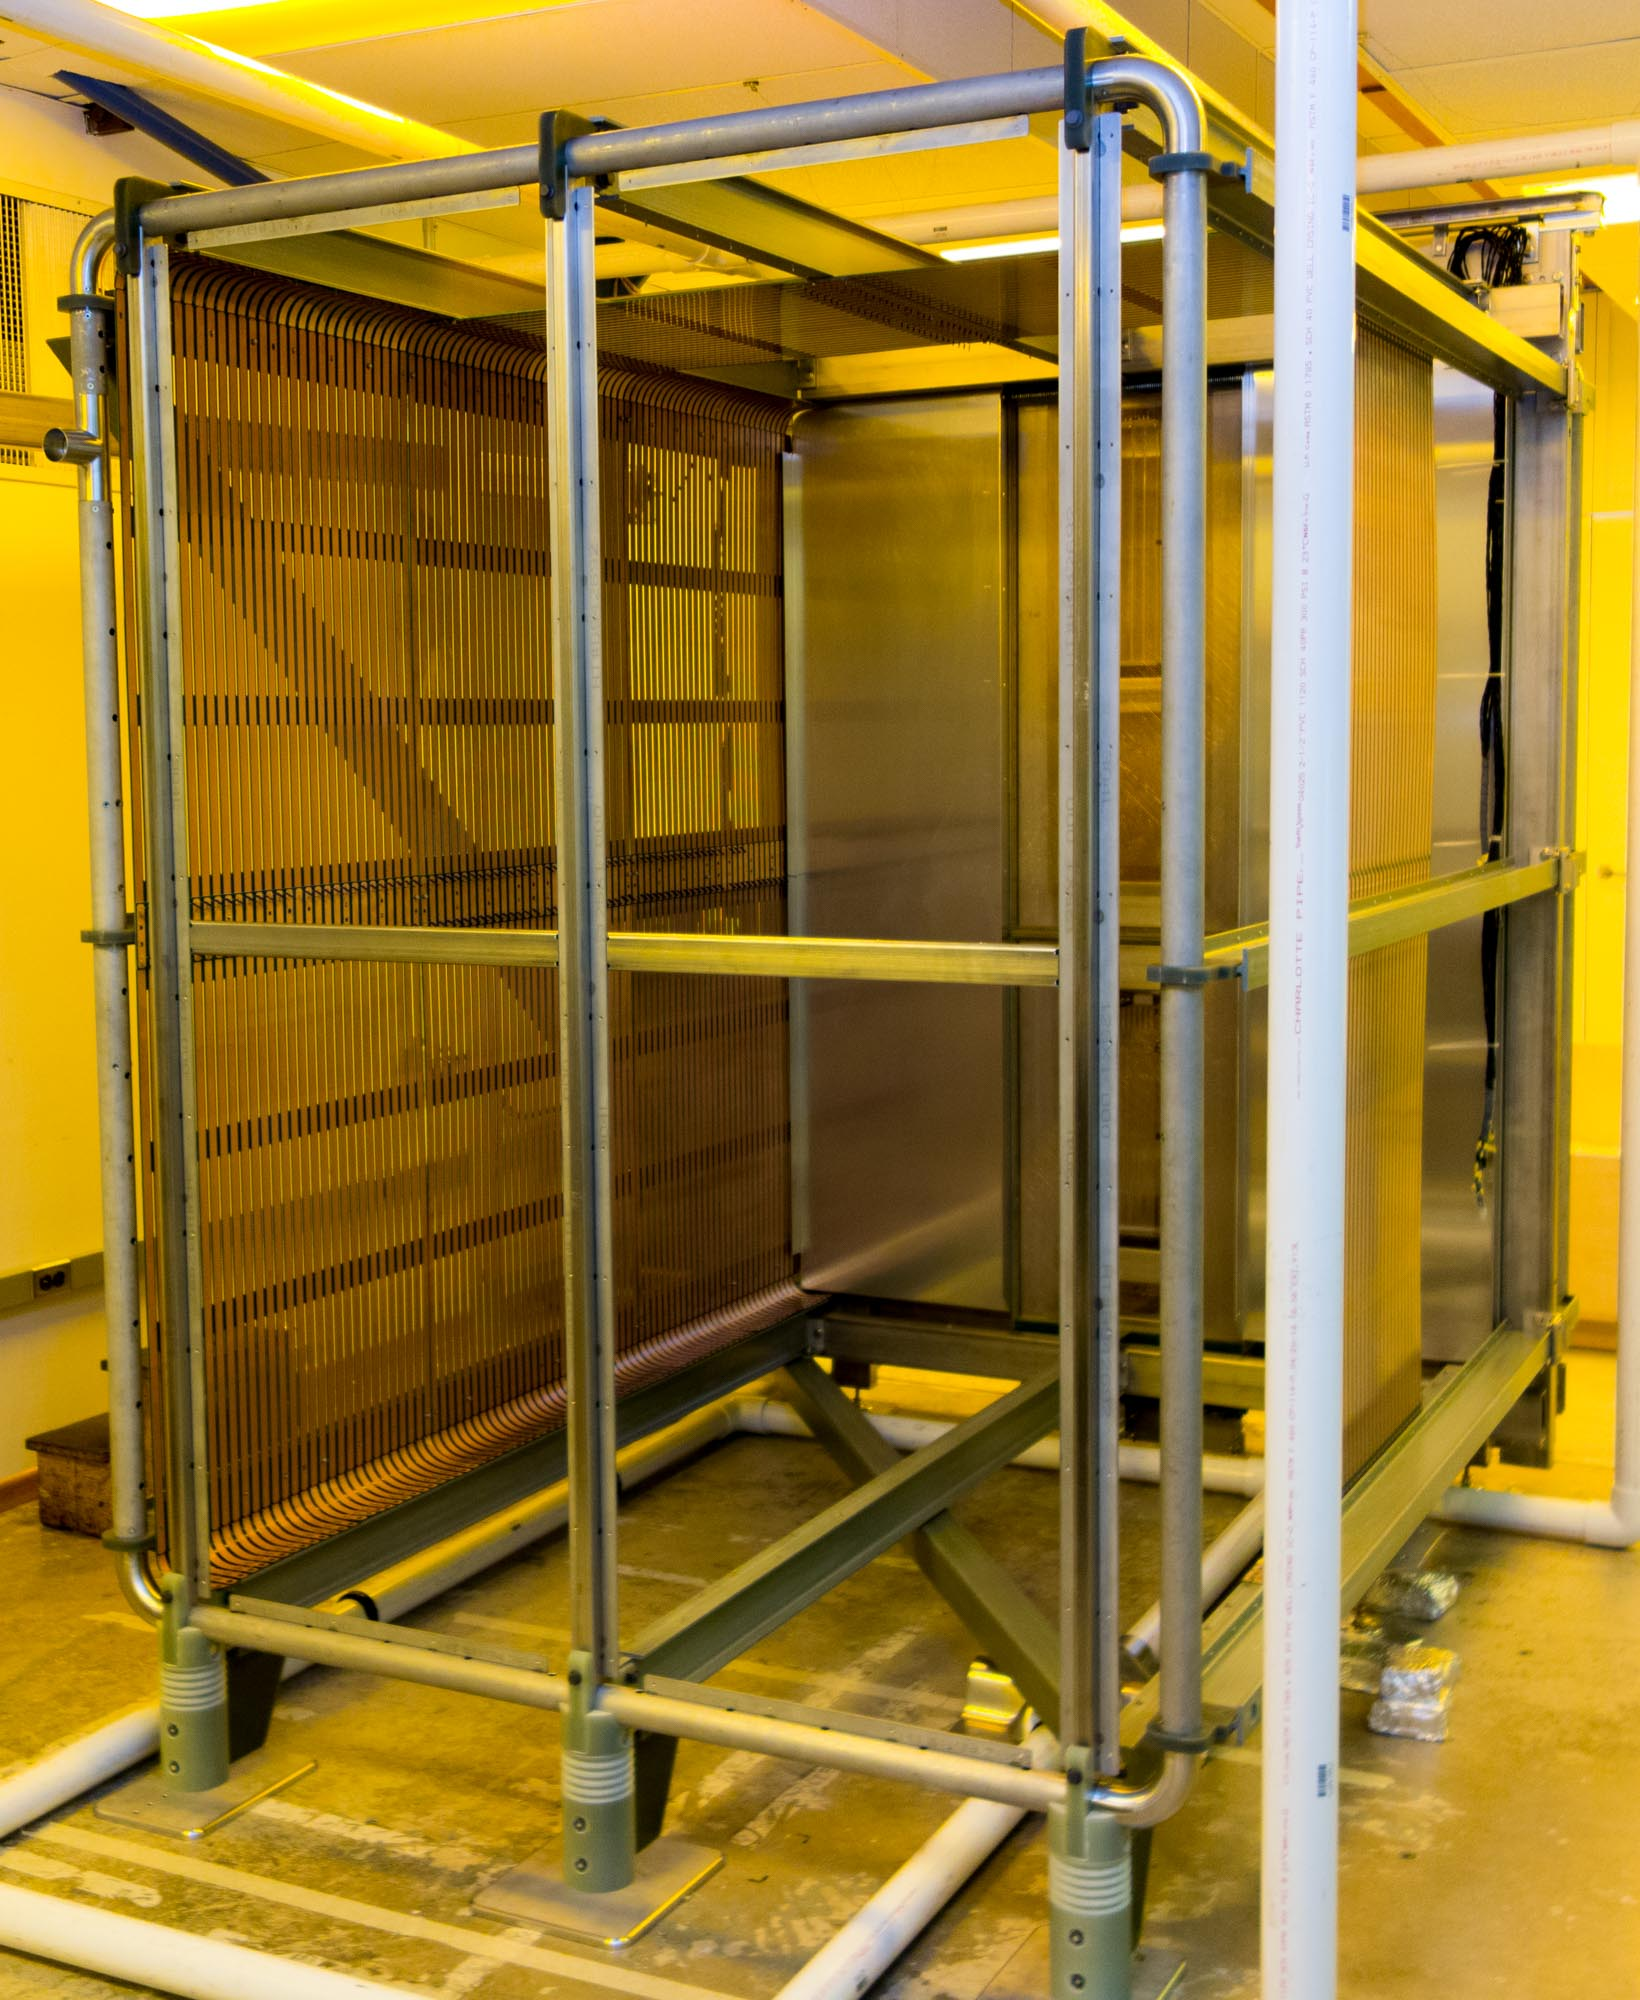
\includegraphics[width=0.35\textwidth]{35TTrial}  
\end{cdrfigure}

The Phase 2 prototype incorporates many of the design elements described in previous
sections of this document.
In many cases, these include novel features that have never previously been tested
in an operational TPC.
Rather than reiterate them all here, some of the more important
aspects are collected in Table~\ref{tab:35TDesign}.

\begin{cdrtable}[35t Design Elements]{lcl}{35TDesign}{35t Design Elements}
 Design Aspect& Section & How Tested\\ \toprowrule
Modular APAs with wrapped wires & \ref{subsec:v5-tpc-chamber-apa}&Build small-scale APA Modules with FD design\\
\colhline
Vertical Gaps between APAs &\ref{subsec:v5-tpc-chamber-apa}& Assemble APAs side-by-side.\\
&&Study reco'd tracks that cross the gaps.\\
\colhline
Horizontal Gaps between APAs &\ref{subsec:v5-tpc-chamber-apa}& Build two shorter APAs and stack vertically\\
&&Study reco'd tracks that cross the gaps\\
\colhline
APAs immersed in active volume &\ref{subsec:v5-tpc-chamber-apa}& Study reco'd tracks that cross APAs\\
\colhline
Cold Digital Electronics & \ref{subsec:fe_CMOS_digital} & Measure noise performance etc. {\it in situ}\\
\colhline
Waveguide-style Photon Detector& \ref{subsec:fe_CMOS_digital}&Install in APAs. Measure lightyield\\
\colhline
Triggerless-capable DAQ & \ref{sec:daq_intro} & Take data using multiple DAQ modes\\ 
\end{cdrtable}

\subsection{Phase 2 Simulation, Reconstruction and Analysis}
As can be seen from Table~\ref{tab:35TDesign}, successful tests of many of the new 
design features requires simulation, reconstruction and analysis of 35t data. 
This will be done with the help of the LarSoft package, which is also used to simulate and 
reconstruct data from the ArgoNeuT and MicroBoone experiments.
Reuse of software developed for those experiments can greatly facilitate 35t development. 
However, the novel hardware features of the 35t prototype necessitate new software developments 
as well.  
Among the required new software developments are:
\begin{itemize}
\item{Code to break up the wrapped wires into as many as five individual linear segments. 
A hit on a single electronic channel can, in principle, be related to an induced signal on any of these segments.}
\item{``Disambiguation'' code to identify which of the possible wire segments was actually responsible
for the observed hit}
\item{Code for determining the start time of the event ($t_0$). Since the 35t prototype DAQ can
run ``triggerless,'' methods are needed for finding the $t_0$ in data. Information from the external 
scintillator paddles as well as the internal photon detectors can be used.}
\item{Code for ``stitching'' together track segments observed in different tracking volumes. 
Since hits can come from either side of the four APAs, there are effectively eight separate tracking volumes, 
which are treated as separate TPCs.}
\end{itemize}

With these simulation and reconstruction tools in hand, ``physics'' analysis of the data can be undertaken.
In addition to the analyses needed to validate the new detector design elements, there are also
some analyses of basic LArTPC performance that are needed as well.
Among the highest priority analysis tasks are:

\begin{itemize}
\item{Basic detector performance: signal/noise, purity measured with tracks, track direction resolution, 
photon detector light yield}
\item{Measurement of distortions due to space charge and field non-uniformity}
\item{Measurements of different types of particles: muons, protons, neutrons, pions}
\end{itemize}

The results obtained by operating the 35t Phase 2 prototype and the analysis of its data are expected
to be very valuable in defining the final far detector design. 

%%%%%%%%%%%%%%%%%%%%%%%%%%%%%%%%%%%%%%%%%%%%%%%%%%%%%%%%%%%%%%%%%%%
\section{Prototype Detector at CERN to Test Physics Sensitivity}

The physics sensitivity of LBNE has been estimated based on detector-performance characteristics published in the literature, simulation-based estimates
and on a variety of assumptions about the anticipated performance of the future detector, event reconstruction and particle-identification algorithms.
A single-phase LAr prototype detector has been proposed for testing in a CERN beam with the goal of
 replacing these assumptions with measurements.  The prototype will implement a full-scale detector element; this will 
 mitigate the risks associated with extrapolating from small-scale versions of the single-phase LAr TPC technology and allow benchmarking of the operation of full-scale detector elements in a well-characterized charged-particle beam.  

The detector will need to accurately identify and measure the energy of the particles produced in the neutrino interaction with argon, which will range from hundreds of MeV to several GeV.
The beam measurements will serve as a calibration data set to tune the Monte Carlo simulations and serve as a reference data set for the detector. 

The prototype is expected to identify any potentially problematic components and lead to future improvements and optimizations of the detector design.


%%%%%%%%%%%%%%%%%%%%%%%%%%%%%%%%%%%%%%%%%%%%%%%%%%%%%%%%%%%%%%%%%%%
% section on other phys expts deleted per Jim Stewart -- it was a hodge podge

%%%%%%%%%%%%%%%%%%%%%%%%%%%%%%%%%%%%%%%%%%%%%%%%%%%%%%%%%%%%%%%%%%%
\section{Summary}

Impressive progress has been made in the development of LArTPC technology over the last few years. All elements of the development program have completed the R\&D phase. Credible conceptual designs exist for all systems in LAr-FD. The technical activities described in this chapter are properly characterized as preliminary engineering design.

The most significant deficiency is the lack of fully-automated event reconstruction. Algorithms have been developed within the LAr community and are being successfully applied to ArgoNeuT data as well as to simulated MicroBooNE data. The algorithms have individually shown that the high efficiency and excellent background rejection capabilities of a LArTPC are achievable. The task remains to combine them into a single package. 


